\documentclass[12pt,a4paper]{article}
\usepackage[utf8]{inputenc}
\usepackage[T1]{fontenc}
\usepackage[spanish]{babel}
\usepackage{geometry}
\usepackage{hyperref}
\usepackage{graphicx}
\usepackage{listings}
\usepackage{xcolor}
\usepackage{booktabs}
\usepackage{tabularx}
\usepackage{array}
\usepackage{caption}
\usepackage{float}
\usepackage{parskip}
\usepackage{enumitem}
\usepackage{titlesec}

\geometry{margin=2.5cm}

% Cambiar "Cuadro" (babel español) por "Tabla"
\addto\captionsspanish{\renewcommand{\tablename}{Tabla}}

% Cambiar "Listing" por "Listado"
\renewcommand{\lstlistingname}{Listado}

\hypersetup{
  colorlinks=true,
  linkcolor=blue!60!black,
  urlcolor=blue!60!black,
  citecolor=blue!60!black
}

\graphicspath{{diagrams/}}

\definecolor{codegray}{rgb}{0.95,0.95,0.95}
\definecolor{codecomment}{rgb}{0.4,0.4,0.4}
\definecolor{codekeyword}{rgb}{0.0,0.3,0.7}
\definecolor{codestring}{rgb}{0.2,0.5,0.2}
\definecolor{codeannotation}{rgb}{0.6,0.3,0.0}
\definecolor{codered}{RGB}{180,30,30}
\definecolor{codegreen}{RGB}{0,120,0}
\definecolor{warnorange}{RGB}{200,100,0}

\lstset{
  language=Java,
  backgroundcolor=\color{codegray},
  basicstyle=\ttfamily\small,
  keywordstyle=\color{codekeyword}\bfseries,
  commentstyle=\color{codecomment}\itshape,
  stringstyle=\color{codestring},
  numbers=left,
  numberstyle=\tiny\color{gray},
  numbersep=8pt,
  breaklines=true,
  showstringspaces=false,
  frame=single,
  framerule=0pt,
  xleftmargin=1em,
  xrightmargin=0.5em,
  captionpos=b,
  extendedchars=true,
  literate=
    {á}{{\'a}}1 {é}{{\'e}}1 {í}{{\'\i}}1 {ó}{{\'o}}1 {ú}{{\'u}}1
    {Á}{{\'A}}1 {É}{{\'E}}1 {Í}{{\'I}}1 {Ó}{{\'O}}1 {Ú}{{\'U}}1
    {ñ}{{\~n}}1 {Ñ}{{\~N}}1 {ü}{{\"u}}1 {Ü}{{\"U}}1
}

\newcommand{\code}[1]{\texttt{#1}}
\newcommand{\clase}[1]{\texttt{#1}}
\newcommand{\metodo}[1]{\texttt{#1}}
\newcommand{\paquete}[1]{\texttt{#1}}
\newcommand{\bad}[1]{\textcolor{codered}{\textbf{#1}}}
\newcommand{\good}[1]{\textcolor{codegreen}{\textbf{#1}}}
\newcommand{\warn}[1]{\textcolor{warnorange}{\textbf{#1}}}

% Columna para tabla de estado de refactorizaciones
\newcolumntype{C}[1]{>{\centering\arraybackslash}m{#1}}

\title{Oportunidades de refactorización en \texttt{org.openmarkov.gui} \\
       \large Catálogo, análisis y plan de ejecución}
\author{OpenMarkov --- CISIAD, UNED}
\date{Abril 2026}

\begin{document}

\maketitle
\tableofcontents
\newpage

% ===================================================================
\section{Introducción}
\label{sec:intro}
% ===================================================================

El módulo \paquete{org.openmarkov.gui} contiene la interfaz gráfica
de escritorio de OpenMarkov: \textasciitilde320 clases y
\textasciitilde59\,000 líneas de código Java (Swing + FlatLaf).
Durante los trabajos de refactorización del núcleo
(\paquete{org.openmarkov.core}) se identificaron múltiples
oportunidades de mejora en la GUI que se documentan aquí.

\textbf{Propósito de este documento:}
\begin{itemize}
  \item Catalogar todas las oportunidades de refactorización detectadas en
        la GUI, con suficiente detalle para ejecutarlas de forma autónoma.
  \item Servir de guía de trabajo: cada sección es una unidad de
        refactorización independiente con estado, ficheros afectados,
        problemas concretos y solución propuesta.
  \item Registrar el progreso de ejecución en la tabla de estado
        (sección~\ref{sec:estado}).
\end{itemize}

% -------------------------------------------------------------------
\subsection{Estructura del módulo}
\label{sec:intro-estructura}
% -------------------------------------------------------------------

La tabla~\ref{tab:paquetes} resume los paquetes principales, su número
de clases y líneas de código.

\begin{table}[H]
\centering
\small
\begin{tabular}{llrr}
\toprule
\textbf{Paquete} & \textbf{Responsabilidad} & \textbf{Clases} & \textbf{Líneas} \\
\midrule
\paquete{window/}               & Paneles principales, controlador  &  5 & 3\,241  \\
\paquete{window/edition/mode/}  & Modos de edición (State pattern)  & 10 &   527   \\
\paquete{graphic/}              & View-model: VisualNode/Link/Net   & 16 & 4\,854  \\
\paquete{dialog/common/}        & Diálogos base + PotentialPanel    & 38 & 8\,706  \\
\paquete{dialog/node/}          & Propiedades de nodo               & 22 & 6\,588  \\
\paquete{dialog/network/}       & Propiedades de red                & 14 & 2\,412  \\
\paquete{dialog/treeadd/}       & Editor TreeADD                   & 20 & 3\,251  \\
\paquete{menutoolbar/}          & Menús y barras de herramientas    & 22 & 6\,252  \\
\paquete{action/}               & PNEdit GUI-específicos (Command)  & 18 & 2\,312  \\
\paquete{component/}            & Tablas de CPT (ValuesTable, etc.) & 20 & 4\,197  \\
\paquete{loader/}               & Iconos y cursores                 & 14 &   879   \\
\paquete{localize/}             & Internacionalización              &  5 &   277   \\
\paquete{validator/}            & Validadores de edición            &  6 &   337   \\
\bottomrule
\end{tabular}
\caption{Paquetes principales de \paquete{org.openmarkov.gui}.}
\label{tab:paquetes}
\end{table}

La figura~\ref{fig:overview} muestra las dependencias entre los
subsistemas principales.

\begin{figure}[H]
\centering
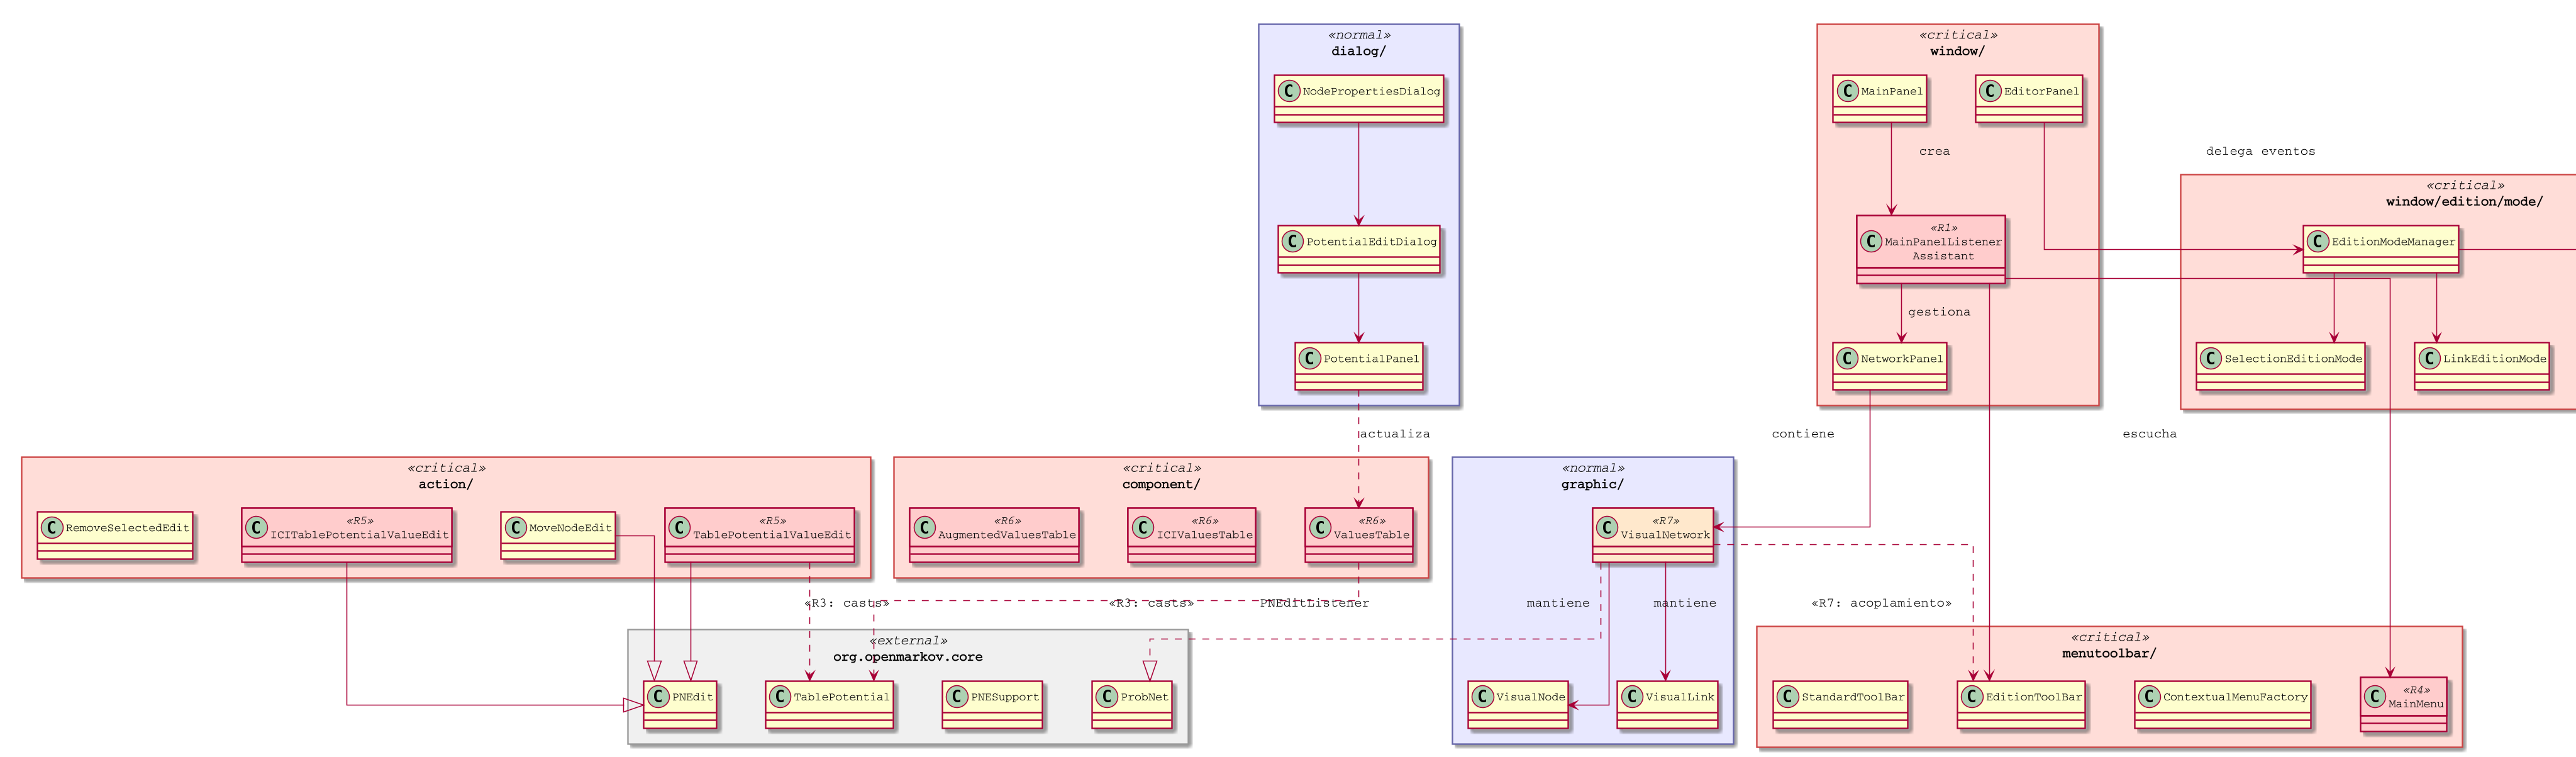
\includegraphics[width=0.95\textwidth]{overview.png}
\caption{Dependencias entre subsistemas de la GUI. Los paquetes en
         \textcolor{codered}{rojo} concentran las oportunidades de
         refactorización más críticas. Diagrama generado con PlantUML
         desde \code{overview.puml}.}
\label{fig:overview}
\end{figure}

% ===================================================================
\section{Estado de las refactorizaciones}
\label{sec:estado}
% ===================================================================

\begin{table}[H]
\centering
\small
\begin{tabular}{C{0.5cm}lC{1.8cm}C{1.5cm}C{1.5cm}}
\toprule
\textbf{\#} & \textbf{Refactorización} & \textbf{Prioridad} & \textbf{Esfuerzo} & \textbf{Estado} \\
\midrule
R1 & Descomposición de \clase{MainPanelListenerAssistant}  & Alta   & Alto     & Completada \\
R2 & Consolidación de modos de creación de nodos           & Alta   & Bajo     & Completada \\
R3 & Eliminación de casts a \clase{TablePotential}         & Media  & Medio    & Completada \\
R4 & Simplificación de \clase{MainMenu}                    & Media  & Medio    & Completada \\
R5 & Consolidación de ediciones de valor en CPT             & Media  & Medio    & Completada \\
R6 & Consolidación de \clase{ValuesTable} y variantes       & Baja   & Alto     & Completada \\
R7 & Simplificación de \clase{VisualNetwork}               & Baja   & Medio    & Completada \\
R8 & Consolidación de editores temporales                   & Baja   & Bajo     & Descartada \\
\bottomrule
\end{tabular}
\caption{Estado de las refactorizaciones. Actualizar la columna
         \emph{Estado} a medida que se ejecutan: Pendiente $\to$
         En curso $\to$ Completada.}
\label{tab:estado}
\end{table}

% ===================================================================
\section{R1 --- Descomposición de \clase{MainPanelListenerAssistant}}
\label{sec:r1}
% ===================================================================

% -------------------------------------------------------------------
\subsection{Situación actual}
% -------------------------------------------------------------------

\clase{MainPanelListenerAssistant} (1\,534 líneas) es el controlador
central de la GUI. Implementa \code{ActionListener} y gestiona \emph{todos}
los eventos de la aplicación a través de un único método
\metodo{actionPerformed()} con \textbf{63 ramas case} en un
\code{switch} sobre \clase{ActionCommands}.

\begin{lstlisting}[caption={Fragmento de \metodo{actionPerformed()} --- 67 ramas case en un único switch}]
@Override public void actionPerformed(ActionEvent e) {
    String actionCommand = e.getActionCommand();
    ActionCommands constant = ActionCommands.of(actionCommand);
    switch (constant) {
        case NEW_NETWORK      -> createNewNetwork();
        case OPEN_NETWORK     -> executeUIAction(this::openNetwork);
        case SAVE_NETWORK     -> executeUIAction(() -> saveNetwork(...));
        case CLIPBOARD_COPY   -> { ... }
        case CLIPBOARD_CUT    -> { ... }
        case UNDO             -> undo();
        case REDO             -> redo();
        case CHANGE_WORKING_MODE -> { ... }
        // ... 50+ ramas más
    }
}
\end{lstlisting}

Adicionalmente, la clase contiene \textbf{12 bloques try-catch}
repartidos en métodos privados. Muchos siguen el patrón mecánico:

\begin{lstlisting}[caption={Patrón repetitivo de try-catch con \clase{UnrecoverableException}}]
private void undo() {
    try {
        undoRedo(true);
    } catch (CannotUndoException e) {
        throw new UnrecoverableException(e);
    }
}
private void redo() {
    try {
        undoRedo(false);
    } catch (CannotRedoException e) {
        throw new UnrecoverableException(e);
    }
}
\end{lstlisting}

El bloque más complejo es el del cambio de modo de trabajo (edición
$\leftrightarrow$ inferencia), con un try-catch anidado de 6 excepciones.

\begin{figure}[H]
\centering
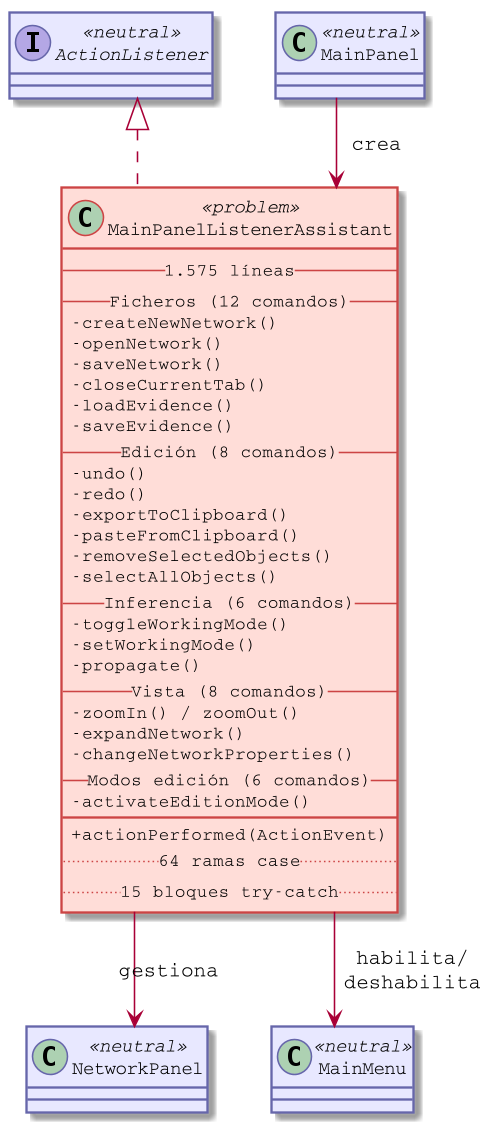
\includegraphics[width=0.5\textwidth]{r1-listener-actual.png}
\caption{Estructura actual de \clase{MainPanelListenerAssistant}:
         clase monolítica que gestiona ficheros, edición, inferencia
         y vista. Diagrama generado desde \code{r1-listener-actual.puml}.}
\label{fig:r1-actual}
\end{figure}

% -------------------------------------------------------------------
\subsection{Problemas}
% -------------------------------------------------------------------

\begin{enumerate}
  \item \bad{Clase God Object}: 1\,534 líneas con responsabilidades
        mezcladas (I/O de ficheros, edición, inferencia, vista, undo/redo).
  \item \bad{Switch monolítico}: 63 ramas case hacen difícil localizar
        y modificar un comportamiento concreto.
  \item \warn{Try-catch mecánicos}: 12 bloques try (23 cláusulas catch)
        cuyo efecto principal es re-envolver excepciones en
        \clase{UnrecoverableException}.
  \item \warn{Acoplamiento}: la clase conoce detalles de diálogos,
        formatos de fichero, algoritmos de inferencia y estado del
        portapapeles.
\end{enumerate}

% -------------------------------------------------------------------
\subsection{Estado: Completada}
% -------------------------------------------------------------------

Descompuesto en fachada ligera + 3~clases delegadas package-private:

\begin{table}[H]
\centering
\small
\begin{tabular}{llr}
\toprule
\textbf{Clase} & \textbf{Responsabilidad} & \textbf{Líneas} \\
\midrule
\clase{MainPanelListenerAssistant} & Fachada: dispatch + API pública & 401 \\
\clase{NetworkFileHandler}         & I/O de ficheros, abrir/guardar/cerrar & 467 \\
\clase{InferenceHandler}           & Modo inferencia, evidencia, propagación & 238 \\
\clase{EditAndViewHandler}         & Undo/redo, zoom, diálogos & 121 \\
\midrule
\textbf{Total}                     & & \textbf{1\,227} \\
\bottomrule
\end{tabular}
\caption{Resultado de la descomposición de \clase{MainPanelListenerAssistant}.
         Original: 1\,534~líneas; reducción neta: $-$307 ($-$20\%).}
\label{tab:r1-delegados}
\end{table}

El beneficio principal es la separación de responsabilidades, no la
reducción de líneas. Se eliminó $\sim$100~líneas de código comentado
muerto.

% -------------------------------------------------------------------
\subsection{Ficheros afectados}
% -------------------------------------------------------------------

\begin{itemize}[nosep]
  \item \code{window/MainPanelListenerAssistant.java} --- fachada (reescritura)
  \item \code{window/NetworkFileHandler.java} --- \textbf{nuevo}
  \item \code{window/InferenceHandler.java} --- \textbf{nuevo}
  \item \code{window/EditAndViewHandler.java} --- \textbf{nuevo}
\end{itemize}

% ===================================================================
\section{R2 --- Consolidación de modos de creación de nodos}
\label{sec:r2}
% ===================================================================

% -------------------------------------------------------------------
\subsection{Estado: Completada}
% -------------------------------------------------------------------

Esta refactorización se ejecutó siguiendo la Opción~A: las tres
subclases (\clase{ChanceNodeEditionMode}, \clase{DecisionNodeEditionMode},
\clase{UtilityNodeEditionMode}) fueron eliminadas.
\clase{NodeEditionMode} es ahora una clase concreta directamente
instanciable que recibe el \code{NodeType} como parámetro del
constructor. \clase{EditionModeManager} registra los tres modos de
nodo programáticamente mediante descriptores
(\code{NODE\_MODE\_DESCRIPTORS}), generando anotaciones
\code{@EditionState} sintéticas para compatibilidad con la toolbar.

% ===================================================================
\section{R3 --- Eliminación de casts a \clase{TablePotential}}
\label{sec:r3}
% ===================================================================

% -------------------------------------------------------------------
\subsection{Situación actual}
% -------------------------------------------------------------------

El módulo GUI contiene \textbf{16 casts explícitos} a
\code{(TablePotential)} y \textbf{10 comprobaciones}
\code{instanceof TablePotential}, distribuidos en 9 ficheros:

\begin{table}[H]
\centering
\small
\begin{tabular}{lcc}
\toprule
\textbf{Fichero} & \textbf{Casts} & \textbf{instanceof} \\
\midrule
\code{action/LinkRestrictionPotentialValueEdit.java}      & 5 & 0 \\
\code{dialog/link/LinkRestrictionPanel.java}              & 4 & 0 \\
\code{action/TablePotentialValueEdit.java}                & 3 & 0 \\
\code{dialog/common/TablePotentialPanel.java}             & 1 & 2 \\
\code{component/ValuesTable.java}                         & 1 & 3 \\
\code{dialog/node/PotentialEditDialog.java}               & 0 & 3 \\
\code{component/LinkRestrictionValuesTable.java}          & 1 & 1 \\
\code{component/PotentialsTablePanelOperations.java}      & 1 & 0 \\
\code{dialog/common/PolicyTypePanel.java}                 & 0 & 1 \\
\midrule
\textbf{Total}                                            & \textbf{16} & \textbf{10} \\
\bottomrule
\end{tabular}
\caption{Distribución de casts e \code{instanceof} a \clase{TablePotential}
         en la GUI. Un total de 26 accesos inseguros.}
\label{tab:r3-casts}
\end{table}

Ejemplo representativo del patrón problemático:

\begin{lstlisting}[caption={Casts encadenados en \clase{LinkRestrictionPotentialValueEdit}}]
// Línea 79
this.tablePotential = (TablePotential) link.getRestrictionsPotential();
this.lastTable = ((TablePotential) link.getRestrictionsPotential())
                     .getValues().clone();
// Línea 92 (en doEdit)
newTable = ((TablePotential) link.getRestrictionsPotential())
               .getValues().clone();
// Línea 100 (en redo)
this.tablePotential = (TablePotential) link.getRestrictionsPotential();
\end{lstlisting}

% -------------------------------------------------------------------
\subsection{Problemas}
% -------------------------------------------------------------------

\begin{enumerate}
  \item \bad{Seguridad de tipos}: si \metodo{getRestrictionsPotential()}
        devuelve otro tipo de \clase{Potential}, se produce un
        \code{ClassCastException} en tiempo de ejecución.
  \item \warn{Duplicación}: el mismo cast se repite 2--5 veces dentro
        de una misma clase.
  \item \warn{Fragilidad}: cualquier cambio en la jerarquía de
        \clase{Potential} exige revisar manualmente los 27 puntos.
\end{enumerate}

% -------------------------------------------------------------------
\subsection{Solución propuesta}
% -------------------------------------------------------------------

Dos líneas de acción complementarias:

\begin{enumerate}
  \item \textbf{Métodos tipados en la API}: donde el contrato garantiza
        que el \clase{Potential} es un \clase{TablePotential} (por
        ejemplo, restricciones de enlace), añadir un método que devuelva
        directamente \code{TablePotential} en \clase{Link}, evitando el
        cast en el lado de la GUI:
\begin{lstlisting}[caption={Método tipado propuesto en \clase{Link}}]
public TablePotential getRestrictionsTablePotential() {
    return (TablePotential) getRestrictionsPotential();
}
\end{lstlisting}
  \item \textbf{Almacenar referencia tipada}: en clases como
        \clase{LinkRestrictionPotentialValueEdit}, hacer el cast una
        sola vez en el constructor y almacenarlo en un campo
        \code{TablePotential}, eliminando los casts redundantes.
\end{enumerate}

% -------------------------------------------------------------------
\subsection{Ficheros afectados}
% -------------------------------------------------------------------

Los 9 ficheros de la tabla~\ref{tab:r3-casts}, más:
\begin{itemize}[nosep]
  \item \code{org.openmarkov.core: model/network/Link.java} --- añadir
        métodos tipados si procede
\end{itemize}

% ===================================================================
\section{R4 --- Simplificación de \clase{MainMenu}}
\label{sec:r4}
% ===================================================================

% -------------------------------------------------------------------
\subsection{Situación actual}
% -------------------------------------------------------------------

\clase{MainMenu} (1\,529 líneas) declara \textbf{53 campos} de tipo
\code{JMenu}/\code{JMenuItem}/\code{JCheckBoxMenuItem} y los
construye imperativamente con \textbf{43 métodos getter} con
inicialización lazy que siguen un patrón repetitivo:

\begin{lstlisting}[caption={Patrón repetitivo de construcción de ítems de menú}]
private JMenuItem getFileNewMenuItem() {
    if (fileNewMenuItem == null) {
        fileNewMenuItem = new LocalizedMenuItem(
            MenuItemNames.FILE_NEW, ActionCommands.NEW_NETWORK);
        fileNewMenuItem.setIcon(IconBind.NEW_ENABLED.icon());
        fileNewMenuItem.setAccelerator(
            KeyStroke.getKeyStroke(KeyEvent.VK_N, CTRL));
        fileNewMenuItem.addActionListener(listener);
    }
    return fileNewMenuItem;
}
// ... x43 métodos casi idénticos
\end{lstlisting}

% -------------------------------------------------------------------
\subsection{Problemas}
% -------------------------------------------------------------------

\begin{enumerate}
  \item \bad{Repetición masiva}: 53 campos y 43 getters lazy con
        estructura idéntica.
  \item \warn{Mantenimiento}: añadir un ítem de menú requiere:
        declarar campo, escribir getter lazy, añadir al menú padre,
        registrar en \clase{MenuItemNames}.
  \item \warn{Tamaño}: 1\,529 líneas dificultan la navegación.
\end{enumerate}

% -------------------------------------------------------------------
\subsection{Estado: Completada}
% -------------------------------------------------------------------

Se reemplazó la construcción imperativa por un
\code{EnumMap<ActionCommands, JComponent>} con métodos factory:

\begin{lstlisting}[caption={Solución aplicada: factory + EnumMap}]
private final Map<ActionCommands, JComponent> items =
    new EnumMap<>(ActionCommands.class);

private void createItem(String name, ActionCommands action,
                        IconBind icon, KeyStroke key) {
    var item = new LocalizedMenuItem(
        name, action.getCommandName(), icon, key);
    item.addActionListener(listener);
    items.put(action, item);
}

// 1 línea por ítem, en vez de 8:
createItem(FILE_NEW_MENUITEM, NEW_NETWORK, NEW_ENABLED, ctrl(VK_N));
\end{lstlisting}

El switch de 43~casos se reemplazó por \code{items.get(cmd)}.
Resultado: 1\,529 $\to$ 425~líneas ($-$72\%).

% -------------------------------------------------------------------
\subsection{Ficheros afectados}
% -------------------------------------------------------------------

\begin{itemize}[nosep]
  \item \code{menutoolbar/menu/MainMenu.java} --- reescritura completa
\end{itemize}

% ===================================================================
\section{R5 --- Consolidación de ediciones de valor en CPT}
\label{sec:r5}
% ===================================================================

% -------------------------------------------------------------------
\subsection{Situación actual}
% -------------------------------------------------------------------

Cuatro clases de edición (\clase{PNEdit}) implementan la lógica de
modificar una celda de una tabla de probabilidad condicional:

\begin{table}[H]
\centering
\small
\begin{tabular}{lr}
\toprule
\textbf{Clase} & \textbf{Líneas} \\
\midrule
\clase{TablePotentialValueEdit}                & 327 \\
\clase{ICITablePotentialValueEdit}             & 429 \\
\clase{AugmentedPotentialValueEdit}            & 205 \\
\clase{LinkRestrictionPotentialValueEdit}      & 175 \\
\midrule
\textbf{Total}                                 & \textbf{1\,136} \\
\bottomrule
\end{tabular}
\caption{Ediciones de valor en CPT con lógica compartida.}
\label{tab:r5-edits}
\end{table}

Las cuatro comparten un patrón común: reciben un \code{Potential},
coordenadas (fila, columna), el valor nuevo, clonan la tabla anterior
en \metodo{doEdit()}, actualizan la celda, y en \metodo{undo()}
restauran la tabla clonada.

\begin{figure}[H]
\centering
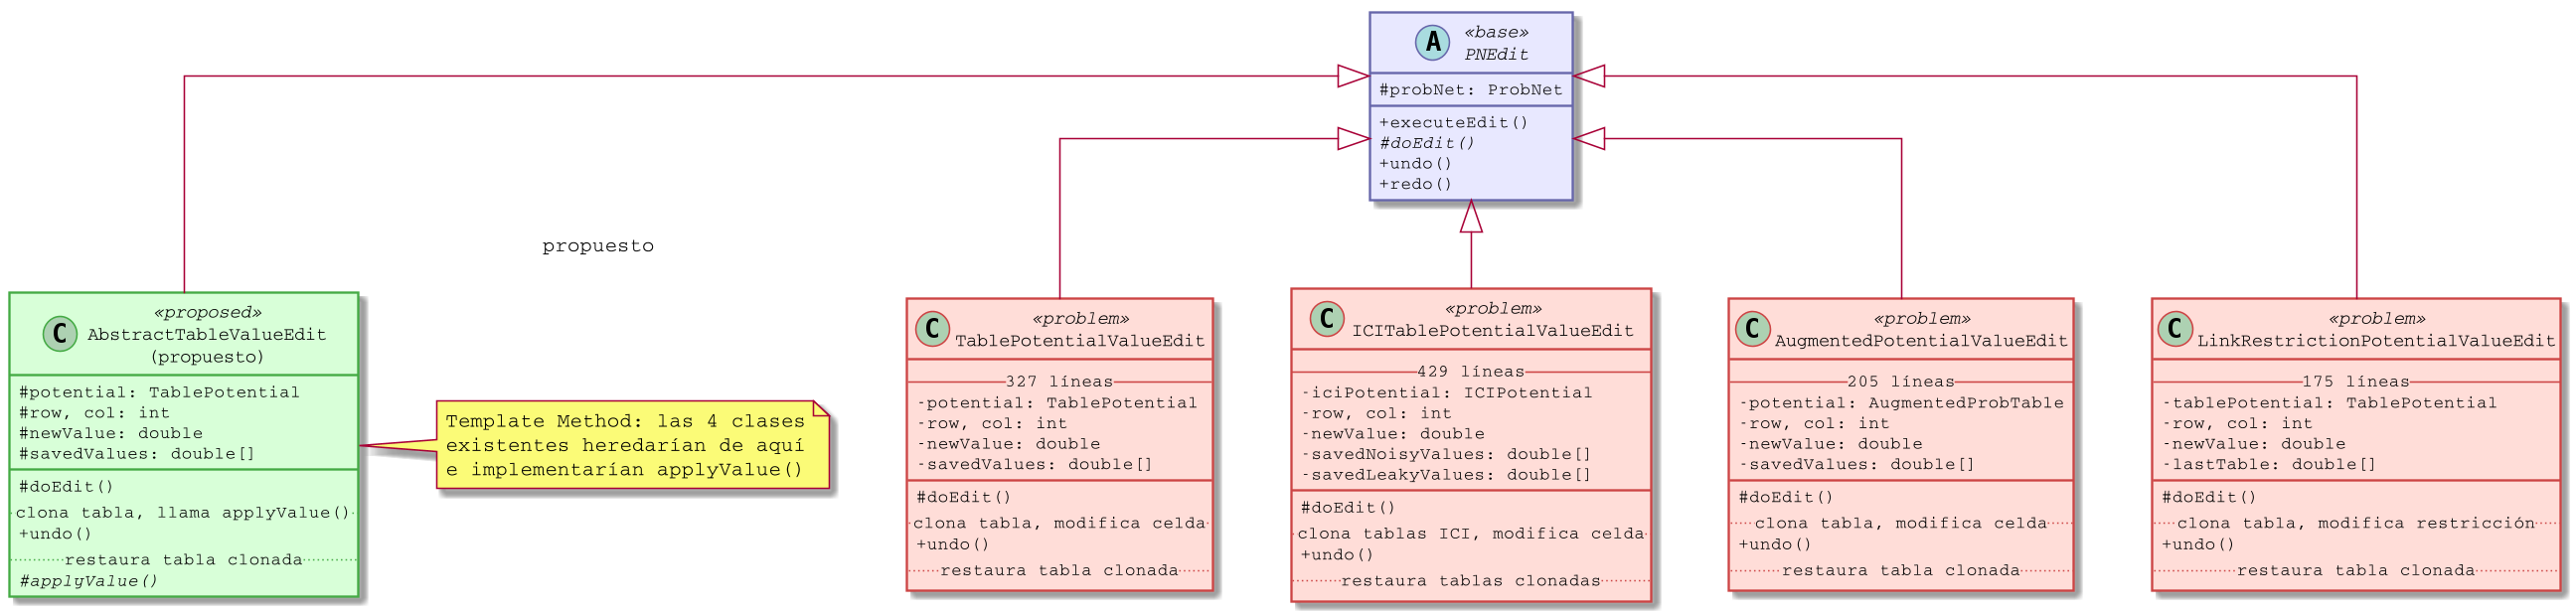
\includegraphics[width=0.85\textwidth]{r5-edits-actual.png}
\caption{Jerarquía actual de las ediciones de valor en CPT.
         Las cuatro clases en rojo comparten la misma estructura
         interna. Diagrama desde \code{r5-edits-actual.puml}.}
\label{fig:r5-actual}
\end{figure}

% -------------------------------------------------------------------
\subsection{Problemas}
% -------------------------------------------------------------------

\begin{enumerate}
  \item \bad{Duplicación}: el algoritmo de redistribución de
        probabilidades (ajustar valores para que sumen~1.0 según
        una lista de prioridad) se repetía en
        \clase{TablePotentialValueEdit} (constructor) e
        \clase{ICITablePotentialValueEdit} (\metodo{doEdit}).
        En esta última, el algoritmo aparecía duplicado internamente
        para parámetros \emph{leaky} y \emph{noisy}.
  \item \warn{Mantenimiento}: un cambio en la lógica de redondeo o
        redistribución debía replicarse en 3~puntos.
\end{enumerate}

% -------------------------------------------------------------------
\subsection{Solución aplicada}
% -------------------------------------------------------------------

La propuesta original de crear una clase base
\clase{AbstractTableValueEdit} resultó inviable porque las cuatro
clases usan dos patrones de herencia incompatibles:
\clase{TablePotentialValueEdit} y \clase{AugmentedPotentialValueEdit}
extienden \clase{PotentialChangeEdit} (reemplazan el potential
entero), mientras que \clase{ICITablePotentialValueEdit} y
\clase{LinkRestrictionPotentialValueEdit} extienden \clase{PNEdit}
directamente. Además, \clase{AugmentedPotentialValueEdit} no usa
redistribución de probabilidades (trabaja con expresiones simbólicas)
y \clase{LinkRestrictionPotentialValueEdit} opera con valores binarios
(0/1) sin normalización.

En su lugar, se extrajo el algoritmo de redistribución a un método
utilitario estático en \clase{PotentialsTablePanelOperations}:

\begin{lstlisting}[caption={Método utilitario de redistribución de probabilidades}]
public static void redistributeProbabilities(
        double[] values, int editedPosition, double newValue,
        List<Integer> priorityList, IntPredicate isEditable)
\end{lstlisting}

El predicado \code{isEditable} permite que
\clase{TablePotentialValueEdit} filtre posiciones no editables
mientras que \clase{ICITablePotentialValueEdit} pasa
\code{pos -> true}.

% -------------------------------------------------------------------
\subsection{Ficheros modificados}
% -------------------------------------------------------------------

\begin{itemize}[nosep]
  \item \code{component/PotentialsTablePanelOperations.java} --- nuevo
        método \metodo{redistributeProbabilities}
  \item \code{action/TablePotentialValueEdit.java} --- eliminadas
        $\sim$40~líneas de redistribución en el constructor
  \item \code{action/ICITablePotentialValueEdit.java} --- eliminadas
        $\sim$70~líneas (dos bloques duplicados leaky/noisy en
        \metodo{doEdit})
\end{itemize}

% ===================================================================
\section{R6 --- Consolidación de \clase{ValuesTable} y variantes}
\label{sec:r6}
% ===================================================================

% -------------------------------------------------------------------
\subsection{Situación actual}
% -------------------------------------------------------------------

El paquete \paquete{component/} contiene una familia de tablas Swing
para edición de CPT:

\begin{table}[H]
\centering
\small
\begin{tabular}{lr}
\toprule
\textbf{Clase} & \textbf{Líneas} \\
\midrule
\clase{ValuesTable}                     & 877 \\
\clase{AugmentedValuesTable}            & 267 \\
\clase{ICIValuesTable}                  & 142 \\
\clase{LinkRestrictionValuesTable}      & 111 \\
\clase{ValuesTableModel}                & 100 \\
\clase{ValuesTableCellRenderer}         & 233 \\
\clase{ICIValuesTableCellRenderer}      & 84  \\
\clase{AugmentedValuesTableCellRenderer}          & 32  \\
\clase{ValuesTableWithLinkRestrictionCellRenderer} & 33  \\
\clase{ValuesTableOptimalPolicyCellRenderer}       & 40  \\
\midrule
\textbf{Total}                          & \textbf{1\,919} \\
\bottomrule
\end{tabular}
\caption{Familia de tablas de CPT en \paquete{component/}.}
\label{tab:r6-tables}
\end{table}

\clase{ValuesTable} (875 líneas) implementa \code{PNEditListener} y
contiene lógica de renderizado, edición y undo/redo. Las variantes
heredan de ella y sobrescriben partes.

% -------------------------------------------------------------------
\subsection{Problemas}
% -------------------------------------------------------------------

\begin{enumerate}
  \item \bad{Clase demasiado grande}: \clase{ValuesTable} con 875 líneas
        mezcla modelo, vista y controlador dentro de un \code{JTable}.
  \item \warn{5 renderers}: la lógica de renderizado está dispersa en
        5 clases separadas con duplicación parcial.
  \item \warn{Herencia frágil}: las variantes dependen de detalles
        internos de \clase{ValuesTable}.
\end{enumerate}

% -------------------------------------------------------------------
\subsection{Estado: Completada}
% -------------------------------------------------------------------

Tras analizar la jerarquía en detalle, las propuestas originales de
consolidación arquitectónica (unificar renderers, extraer
\code{PNEditListener}, reemplazar herencia por configuración) se
descartaron por riesgo alto y beneficio limitado:

\begin{itemize}[nosep]
  \item Los 5~renderers implementan lógica de coloreado genuinamente
        diferente (ICI, política óptima, restricciones de enlace).
  \item Los callbacks \code{PNEditListener} están acoplados al modelo
        de datos de cada tabla (posiciones fila/columna de ediciones
        específicas).
  \item Las subclases usan correctamente template method: cada una
        sobreescribe \code{setValueAt()} y \code{afterEditExecutes()}
        con tipos de edición fundamentalmente distintos.
\end{itemize}

En su lugar, se realizó limpieza de código muerto y correcciones
puntuales:

\begin{itemize}[nosep]
  \item \textbf{Clase eliminada}: \clase{AugmentedValuesTableCellRenderer}
        (32~líneas) --- nunca instanciada.
  \item \textbf{AugmentedValuesTable}: eliminados \code{printTable()},
        \code{editCellAt()} (debug con \code{System.err.println}),
        \code{selectAll()} (copia privada inalcanzable) --- $-$84~líneas.
  \item \textbf{ValuesTable}: eliminado \code{printTable()} --- método
        debug nunca invocado --- $-$21~líneas.
  \item \textbf{ICIValuesTable}: eliminado campo \code{lastCol} que
        sombreaba el campo \code{protected} del padre --- $-$4~líneas.
  \item \textbf{LinkRestrictionCellRenderer}: eliminado parámetro
        \code{TablePotential} no utilizado. Actualizados 3~puntos de
        llamada en \clase{LinkRestrictionPanel}.
  \item \textbf{LinkRestrictionValuesTable}: eliminada variable local
        \code{net} y \code{node1} no utilizadas --- $-$9~líneas.
\end{itemize}

\textbf{Resultado}: 1\,461 $\to$ 1\,309~líneas ($-$152), 1~clase
eliminada.

% ===================================================================
\section{R7 --- Simplificación de \clase{VisualNetwork}}
\label{sec:r7}
% ===================================================================

% -------------------------------------------------------------------
\subsection{Situación actual}
% -------------------------------------------------------------------

\clase{VisualNetwork} (1\,172 líneas) es la clase view-model que
mantiene la representación visual de la red. Implementa
\code{PNEditListener} y, en respuesta a cualquier edición, reconstruye
toda la estructura visual:

\begin{lstlisting}[caption={Métodos \code{PNEditListener} en \clase{VisualNetwork}}]
@Override public void afterEditExecutes(PNEdit edit) {
    constructVisualInfo();
    if (getWorkingMode() != NetworkEditorPanel.WorkingMode.INFERENCE) {
        visualDecisionNodeRefresh();
    }
    mainGUI.mainPanel.getEditionToolBar().getUndoButton()
           .setEnabled(probNet.getPNESupport().getCanUndo());
    mainGUI.mainPanel.getEditionToolBar().getRedoButton()
           .setEnabled(probNet.getPNESupport().getCanRedo());
}

@Override public void afterUndoingEdit(PNEdit edit) {
    refreshUI();  // mismo cuerpo que afterEditExecutes
}

@Override public void afterRedoingEdit(PNEdit edit) {
    refreshUI();  // mismo cuerpo que afterEditExecutes
}
\end{lstlisting}

% -------------------------------------------------------------------
\subsection{Problemas}
% -------------------------------------------------------------------

\begin{enumerate}
  \item \warn{Acoplamiento ascendente}: \clase{VisualNetwork} (capa
        view-model) accede directamente a
        \code{mainGUI.mainPanel.getEditionToolBar()} (capa UI), violando
        la dirección de dependencias del MVC.
  \item \warn{Reconstrucción total}: \metodo{constructVisualInfo()}
        reconstruye todos los nodos y arcos visuales ante cualquier
        edición, sin distinguir qué cambió.
  \item \warn{Tamaño}: 1\,177 líneas combinan mantenimiento de
        colecciones, geometría, hit-testing y notificación.
\end{enumerate}

% -------------------------------------------------------------------
\subsection{Estado: Completada}
% -------------------------------------------------------------------

Se eliminó el campo \code{mainGUI} de \clase{VisualNetwork} y las 4
líneas que manipulaban directamente los botones undo/redo de
\clase{EditionToolBar}. La actualización de estos botones ya la realiza
\clase{MainPanelMenuAssistant} mediante su método
\code{updateUndoRedo()}, que invoca
\code{setOptionEnabled(ActionCommands.UNDO/REDO, ...)}. Este método,
heredado de \clase{MenuAssistant}, itera sobre todas las
implementaciones de \code{MenuToolBarBasic} registradas --- incluyendo
tanto \clase{MainMenu} como las clases de toolbar --- por lo que los
botones de toolbar ya se actualizaban por esta vía.

El constructor de \clase{VisualNetwork} pasó de
\code{VisualNetwork(ProbNet, MainGUI)} a \code{VisualNetwork(ProbNet)}.
Se actualizó el único punto de llamada en \clase{NetworkEditorPanel}.

No fue necesario registrar \clase{EditionToolBar} como
\code{PNEditListener} independiente, ya que el mecanismo existente en
\clase{MainPanelMenuAssistant} cubre tanto menús como toolbars.

\begin{itemize}[nosep]
  \item \code{graphic/VisualNetwork.java} --- 1\,172 $\to$ 1\,161 líneas ($-$11)
  \item \code{window/edition/NetworkEditorPanel.java} --- eliminado argumento
        \code{mainGUI} en constructor de \clase{VisualNetwork}
\end{itemize}

% ===================================================================
\section{R8 --- Consolidación de editores temporales}
\label{sec:r8}
% ===================================================================

% -------------------------------------------------------------------
\subsection{Situación actual}
% -------------------------------------------------------------------

Tres clases de edición gestionan intervalos temporales con estructura
similar:

\begin{table}[H]
\centering
\small
\begin{tabular}{lr}
\toprule
\textbf{Clase} & \textbf{Líneas} \\
\midrule
\clase{NodePartitionedIntervalEdit}   & 165 \\
\clase{RevelationIntervalEdit}        & 152 \\
\clase{PartitionedIntervalEdit}       & 47  \\
\midrule
\textbf{Total}                        & \textbf{364} \\
\bottomrule
\end{tabular}
\caption{Ediciones temporales con estructura compartida.}
\label{tab:r8-temporal}
\end{table}

Las tres manipulan rangos temporales (\code{timeSlice}) sobre nodos
y comparten la lógica de validación de intervalos y undo.

% -------------------------------------------------------------------
\subsection{Problemas}
% -------------------------------------------------------------------

\begin{enumerate}
  \item \warn{Duplicación parcial}: la validación de intervalos y la
        lógica de undo se repite con variaciones menores.
  \item \warn{Baja prioridad}: el volumen total es pequeño (364 líneas)
        y la duplicación es parcial, no total.
\end{enumerate}

% -------------------------------------------------------------------
\subsection{Decisión: descartada}
% -------------------------------------------------------------------

Tras analizar el código, las tres clases no comparten suficiente
estructura para justificar una abstracción común:
\clase{PartitionedIntervalEdit} (47~líneas) es un simple swap de
intervalos; \clase{NodePartitionedIntervalEdit} modifica propiedades
in-place; \clase{RevelationIntervalEdit} manipula una lista en un
link con 4~acciones distintas (ADD, REMOVE, MODIFY\_VALUE,
MODIFY\_DELIMITER). Los modelos de datos y las estrategias de backup
son incompatibles. La duplicación parcial no justifica el coste de
una abstracción para 364~líneas.

% ===================================================================
\section{Orden de ejecución recomendado}
\label{sec:orden}
% ===================================================================

Las refactorizaciones se han ordenado considerando: (1) impacto en
mantenibilidad, (2) riesgo de regresión, (3) dependencias entre
ellas.

\begin{enumerate}
  \item \textbf{R2} --- \good{Completada}. Las tres subclases fueron
        eliminadas y \clase{NodeEditionMode} es ahora instanciable
        directamente.
  \item \textbf{R3} (casts TablePotential) --- \good{Completada}.
        Cambiada la firma de \metodo{Link.getRestrictionsPotential()}
        para devolver \clase{TablePotential}; eliminados 15 de 16
        casts con pattern matching \code{instanceof}.
  \item \textbf{R5} (ediciones de valor CPT) --- \good{Completada}.
        Extraído algoritmo de redistribución de probabilidades a
        \metodo{PotentialsTablePanelOperations.redistributeProbabilities};
        eliminadas $\sim$110~líneas duplicadas.
  \item \textbf{R8} (editores temporales) --- \warn{Descartada}.
        Las 3~clases no comparten suficiente estructura para
        justificar una abstracción (ver \S\ref{sec:r8}).
  \item \textbf{R4} (MainMenu) --- \good{Completada}.
        53~campos y 46~getters lazy reemplazados por
        \code{EnumMap<ActionCommands, JComponent>} con métodos factory;
        switch de 43~casos reemplazado por \code{items.get(cmd)};
        1\,529 $\to$ 425~líneas ($-$72\%).
  \item \textbf{R1} (MainPanelListenerAssistant) --- \good{Completada}.
        Descompuesto en fachada (401~líneas) + 3~handlers
        package-private: \clase{NetworkFileHandler} (467),
        \clase{InferenceHandler} (238), \clase{EditAndViewHandler}~(121).
  \item \textbf{R7} (VisualNetwork) --- \good{Completada}.
        Eliminado campo \code{mainGUI} y acceso directo a toolbar;
        la actualización undo/redo ya la gestiona
        \clase{MainPanelMenuAssistant}.
  \item \textbf{R6} (ValuesTable) --- \good{Completada}.
        Limpieza de código muerto: 1~clase eliminada, métodos debug,
        campo sombreado, parámetro no utilizado; $-$152~líneas.
        Consolidación arquitectónica descartada por alto riesgo.
\end{enumerate}

\begin{figure}[H]
\centering
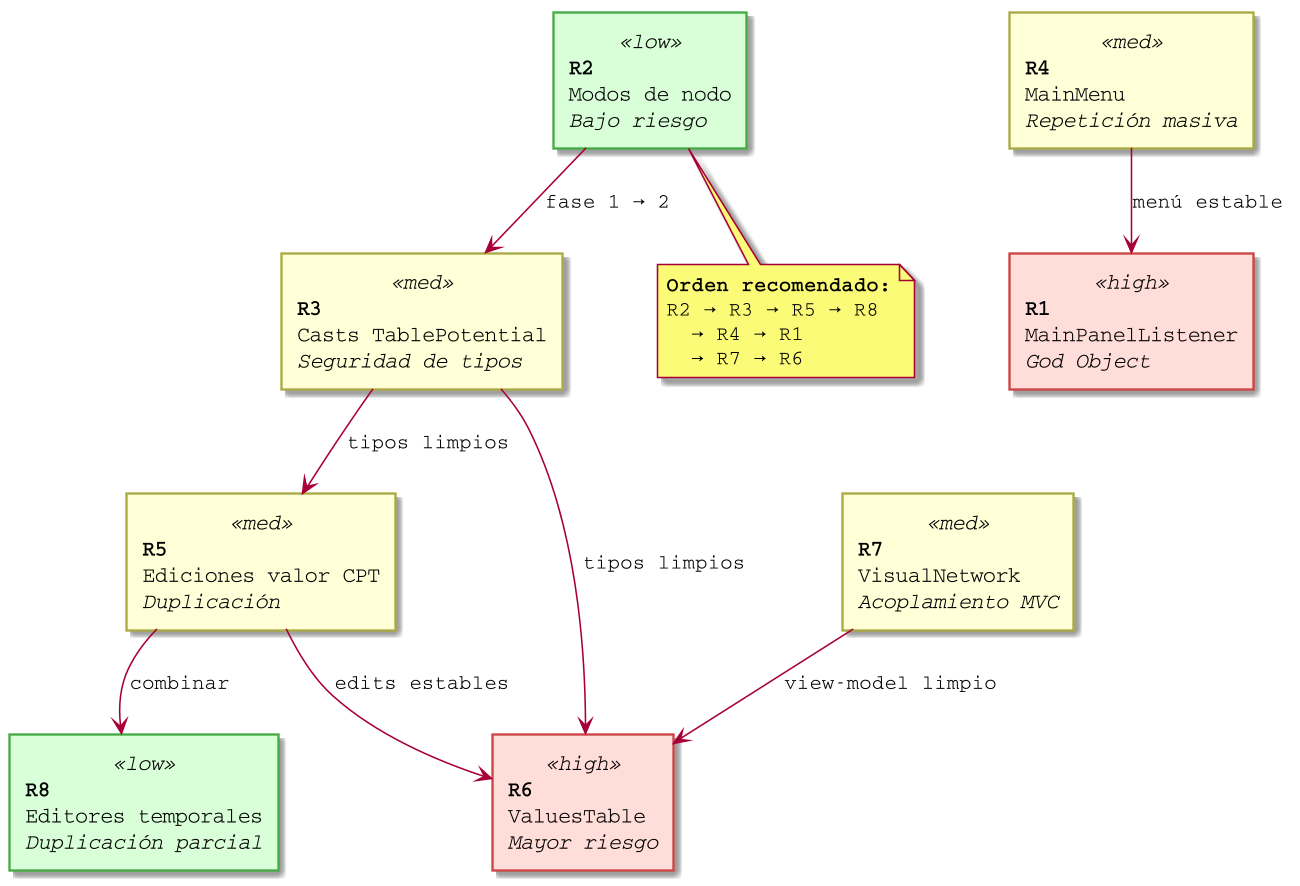
\includegraphics[width=0.75\textwidth]{orden-ejecucion.png}
\caption{Grafo de dependencias entre refactorizaciones. Las flechas
         indican ``debería hacerse antes de''. Diagrama desde
         \code{orden-ejecucion.puml}.}
\label{fig:orden}
\end{figure}

% ===================================================================
\section{Resumen cuantitativo}
\label{sec:resumen}
% ===================================================================

\begin{table}[H]
\centering
\small
\begin{tabular}{lrrrl}
\toprule
\textbf{Refact.} & \textbf{Clases} & \textbf{Líneas} & \textbf{Reducción est.} & \textbf{Beneficio principal} \\
\midrule
R1 & 4  & 1\,534  & $-$307   & \good{Completada}                 \\
R2 & 5  &    527  & $-$44    & \good{Completada}                 \\
R3 & 10 & 2\,500  & $-$200   & \good{Completada}                 \\
R4 & 1  & 1\,529  & $-$1\,104 & \good{Completada}                 \\
R5 & 3  & 1\,136  & $-$110   & \good{Completada}                 \\
R6 & 7  & 1\,461  & $-$152   & \good{Completada}                 \\
R7 & 2  & 1\,172  & $-$11    & \good{Completada}                 \\
R8 & 3  &    364  &     0    & \warn{Descartada}                 \\
\midrule
\textbf{Total} & \textbf{34} & \textbf{10\,223} & \textbf{$-$1\,517} & \\
\bottomrule
\end{tabular}
\caption{Resumen cuantitativo de las refactorizaciones propuestas.
         La columna ``Reducción est.'' indica la reducción estimada
         en líneas de código (neto, sin contar nuevas clases base).}
\label{tab:resumen}
\end{table}

\end{document}
